\documentclass{beamer}
\usepackage{xunicode}
\usepackage{fontspec}
\usepackage{graphicx}
\usepackage[english]{babel}
\renewcommand{\familydefault}{\sfdefault}

\usetheme{CambridgeUS}
%\usecolortheme{beaver}




%\definecolor{titre}{rgb}{0.50,0.00,0.10}
%\setbeamercolor{structure}{fg=titre, bg=white}

\setbeamertemplate{navigation symbols}{}
%\setbeamertemplate{footline}{\hfill\insertframenumber/\inserttotalframenumber}

\AtBeginSection[]
{
    \begin{frame}
        \frametitle{Questions?}
    \end{frame}

	\frame{
		\frametitle{What now?}
%		\tableofcontents[currentsection,hideothersubsections]
        \tableofcontents[sectionstyle=show/shaded, subsectionstyle=show/show/hide]
	}
}


\title{Git : model and workflows}
\author{Julien Durillon}
\institute{Clever Cloud}
\date{\today}

\begin{document}
	\frame{\titlepage}

	\frame{
		\frametitle{Table of Contents}
		\tableofcontents[sectionstyle=show/show, subsectionstyle=hide/hide]
	}

	\section{Introduction}
	\begin{frame}
	    \frametitle{Introduction}
	    \begin{itemize}
            \item Hard to manage all the commands?
            \item What does checkout do ? \pause
            \item to revert unstaged changes\pause
            \item Set a file in an old state\dots \pause
            \item of a commit, of a tag, of a branch
	    \end{itemize}
	\end{frame}


	\section{Objects}

	\begin{frame}
        \frametitle{Git objects}
        \framesubtitle{What do they all look like?}
        \begin{minipage}{0.5\textwidth}
        \begin{center}
            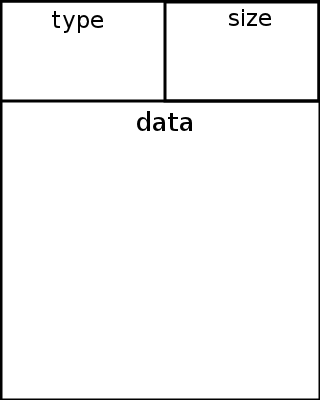
\includegraphics[width=0.6\textwidth]{./figures/object.png}
        \end{center}
        \end{minipage}
        \begin{minipage}{0.4\textwidth}
        Addressed by a SHA1 identifier calculated from the whole content of the object.
        \end{minipage}
	\end{frame}

	\subsection{User objects}

	\begin{frame}
	    \frametitle{Blobs and Trees}
	    \framesubtitle{Basically\dots}
	    \begin{center}
        \begin{itemize}
            \item A blob is a file
            \item A tree is a folder
        \end{itemize}
        \end{center}
    \pause
        \begin{center}
            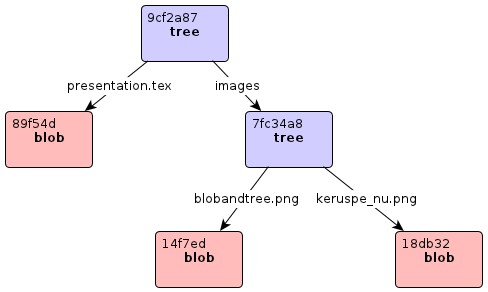
\includegraphics[height=0.5\textheight]{./figures/blobandtree.png}
        \end{center}
	\end{frame}


    \subsection{Commits}

    \begin{frame}
	    \frametitle{Commits}
	    \framesubtitle{Contain}
	        \begin{itemize}
	            \item Author \onslide<2->{ -- The one who wrote the code}
                \item Commiter \onslide<3->{ -- The one who created the commit object}
                \item Parent \onslide<4->{ -- The commit(s) before this one}
                \item Tree \onslide<5->{ -- The top tree object of the commited state}
                \item Message \onslide<6->{ -- Why the commit was done}
	        \end{itemize}
	\end{frame}

    \subsection{Storage}

    \begin{frame}[fragile]
	    \frametitle{Storage}
	    \framesubtitle{What does .git look like?}
        \begin{verbatim}
.git
|-- config
|-- description
|-- HEAD
|-- hooks
|-- info
|-- objects
`-- refs
        \end{verbatim}
	\end{frame}

	\begin{frame}[fragile]
	    \frametitle{Storage}
	    \framesubtitle{"We need to go deeper"}
\begin{verbatim}
.git/objects
|-- 10
|   `-- 8c8bff3b82234d1726531c6643cbb541d4bc4e
|-- 42
|   `-- 0f12c08fcb785df9d8c1887e2545882d6168ea
|-- 5c
|   `-- 4b717a0ea3b0c100c5e4141da431014253d44b
|-- info
`-- pack
\end{verbatim}
\pause
\begin{verbatim}
.git/refs
|-- heads
|   `-- master
`-- tags
\end{verbatim}
	\end{frame}

	\subsection{Examples}

    \begin{frame}
        \frametitle{Example}
        \framesubtitle{Plumbing tools}

        \begin{itemize}
            \item hash-object
            \item cat-file
        \end{itemize}

    \end{frame}

	\subsection{Branches, Tags, all that stuff}

    \begin{frame}
        \frametitle{Only ``labels"}
        \framesubtitle{No working tree copy}

        A simple project:

        \begin{center}
            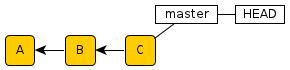
\includegraphics[width=0.5\textwidth]{figures/branches1.png}
        \end{center}
        \pause
        A less simple project:
        \begin{center}
            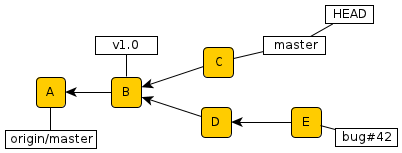
\includegraphics[width=0.7\textwidth]{figures/branches2.png}
        \end{center}

    \end{frame}


    \subsection{Back to checkout}

    \begin{frame}
        \frametitle{Back to checkout}
        \begin{center}
            Does one thing: get a file/tree in the state of a commit.
        \end{center}
    \end{frame}

    \section{Remotes}

    \subsection{Storing the remotes}
    \begin{frame}
        \frametitle{Storing the remotes}

        \begin{itemize}
            \item In .git/refs/remotes
            \item points to a commit like a branch or a tag
            \item can't and shouldn't be changed by other than fetch
        \end{itemize}

    \end{frame}

    \subsection{Understanding the remotes}

    \begin{frame}
        \frametitle{Understanding remotes}
        \begin{center}
            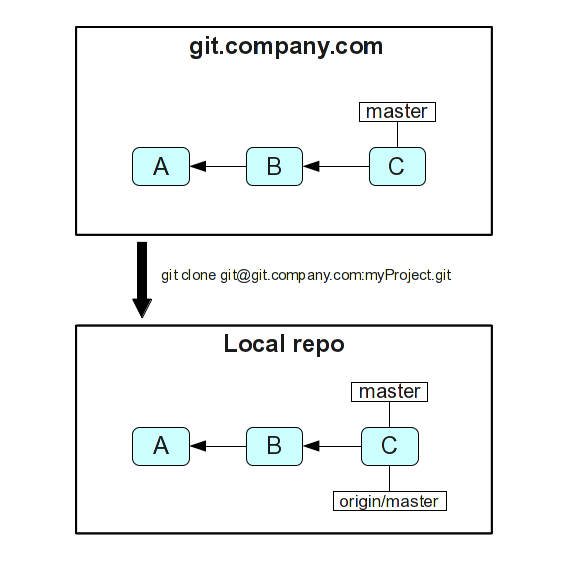
\includegraphics[width=0.6\textwidth]{figures/clone.png}
        \end{center}
    \end{frame}

    \begin{frame}
    \frametitle{Understanding remotes}
    \begin{minipage}{0.5\textwidth}
        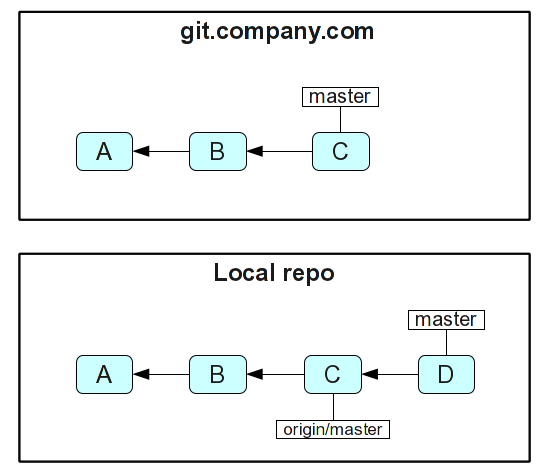
\includegraphics[width=\textwidth]{figures/after-commit.png}
    \end{minipage}
    \begin{minipage}{0.4\textwidth}
    \footnotesize
\# On branch master\\
\# Your branch is ahead of\\
\# 'origin/master' by 1 commit.\\
\# \\
nothing to commit (working directory clean)
    \end{minipage}
    \end{frame}


    \begin{frame}
        \frametitle{Understanding remotes}
        \begin{center}
            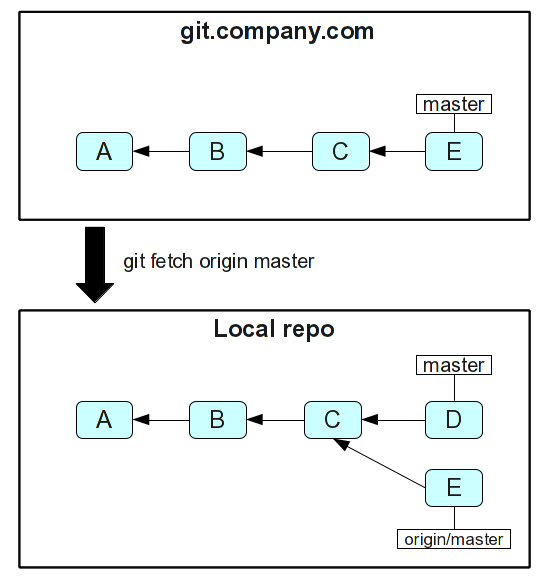
\includegraphics[width=0.6\textwidth]{figures/re-fetch.png}
        \end{center}
    \end{frame}


    \section{Workflows}

        \subsection{Basic "recommended" usage}

    \begin{frame}
        \frametitle{Fully decentralized: the official way}
        \begin{center}
            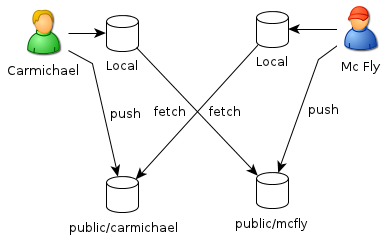
\includegraphics[width=0.8\textwidth]{./figures/repo-official.png}
        \end{center}

    \end{frame}

    \begin{frame}
        \frametitle{Fully decentralized: limitations}
        \begin{center}
            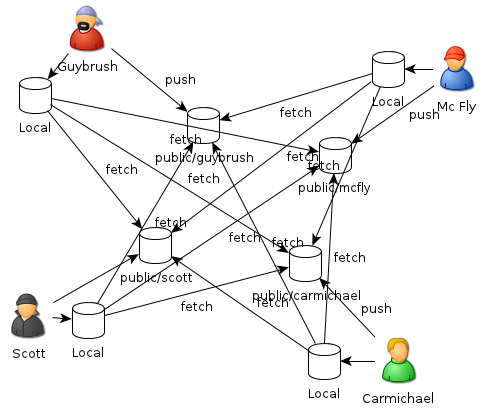
\includegraphics[width=0.7\textwidth]{./figures/decent-wf-fail.png}
        \end{center}

    \end{frame}

        \subsection{Centralized: à la Subversion}

    \begin{frame}
        \frametitle{Centralized: à la Subversion}
        \begin{center}
            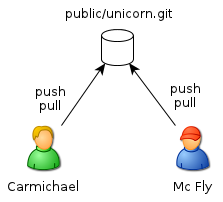
\includegraphics[width=0.5\textwidth]{./figures/svnstyle.png}
        \end{center}
    \end{frame}

        \subsection{Big project: The benevolent dictator}
    \begin{frame}
        \frametitle{The benevolent dictator}
        \begin{center}
            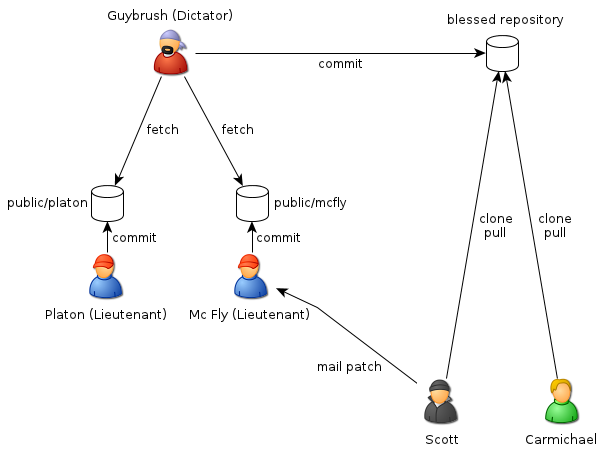
\includegraphics[width=0.8\textwidth]{./figures/dictator.png}
        \end{center}

    \end{frame}

\end{document}

